%!TEX root = ../dissertation.tex

\chapter{Implementation}
\label{chapter:implementation}
Chapter~\ref{chapter:implementation} describes the implementation details for the solution that was
presented in Chapter~\ref{chapter:solution}. Here we described the technological components of our
smart warehouse for the proposed approaches, as well we describe the implementation details and
technological details for the provisioning mechanism.

% Smart Warehouse Deployment
\section{Smart Warehouse Deployment}
\label{sec:Smart Place}
The smart warehouse setup was based in a real scenario described by Correia et al. \cite{correiaalpharfid},
as illustrated in Figure~\ref{fig:rfidapp_setup}.\\

% RFID application setup
\begin{figure}[ht!]
  \centering
  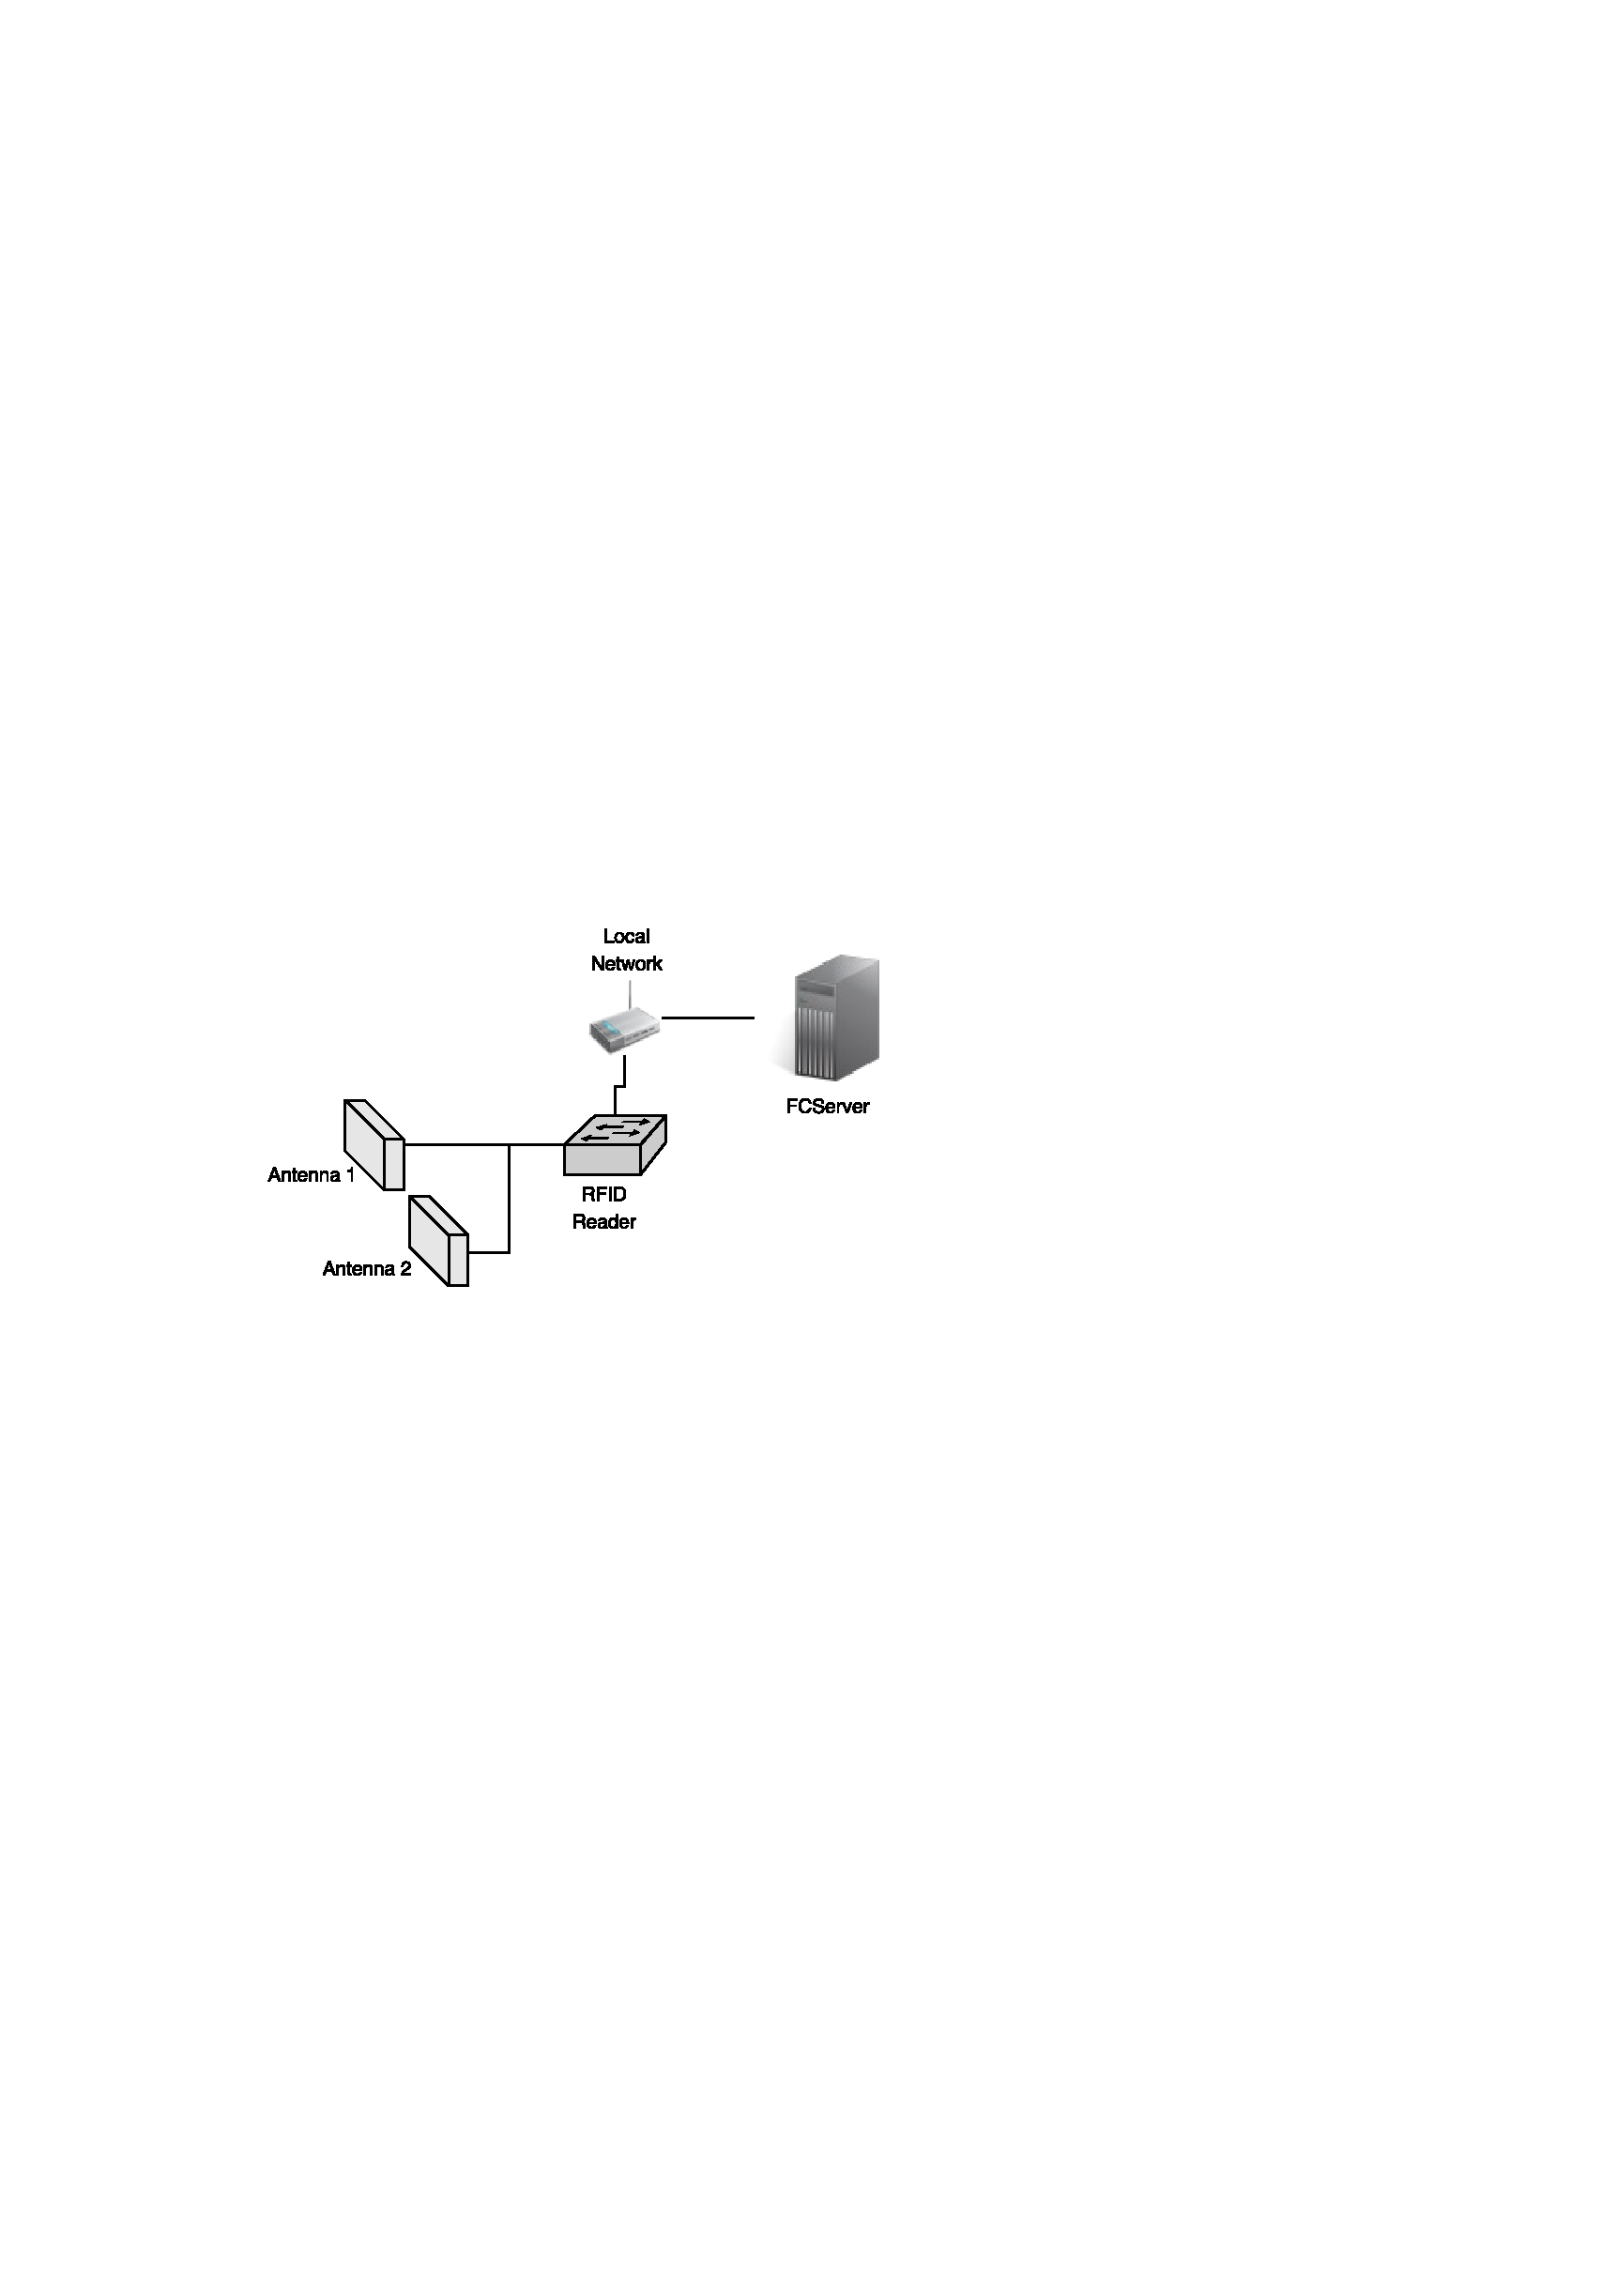
\includegraphics[width=.6\textwidth]{./images/rfidapp_setup}
  \caption{RFID application setup.}
  \label{fig:rfidapp_setup}
\end{figure}

The warehouse is composed of a tagged robot that is identified by \gls{RFID} readers that are deployed
in the physical space. To monitoring the robot inside the warehouse, we decide to use the Fosstrak
\gls{RFID} middleware. The communication between the middleware and the \gls{RFID} readers is performed
through the \gls{LLRP} protocol.

% Cloud approach
\subsection{Cloud Deployment}
\label{sub:imp_smart_warehouse_cloud}

% Cloud approach
\begin{figure}[ht!]
  \centering
  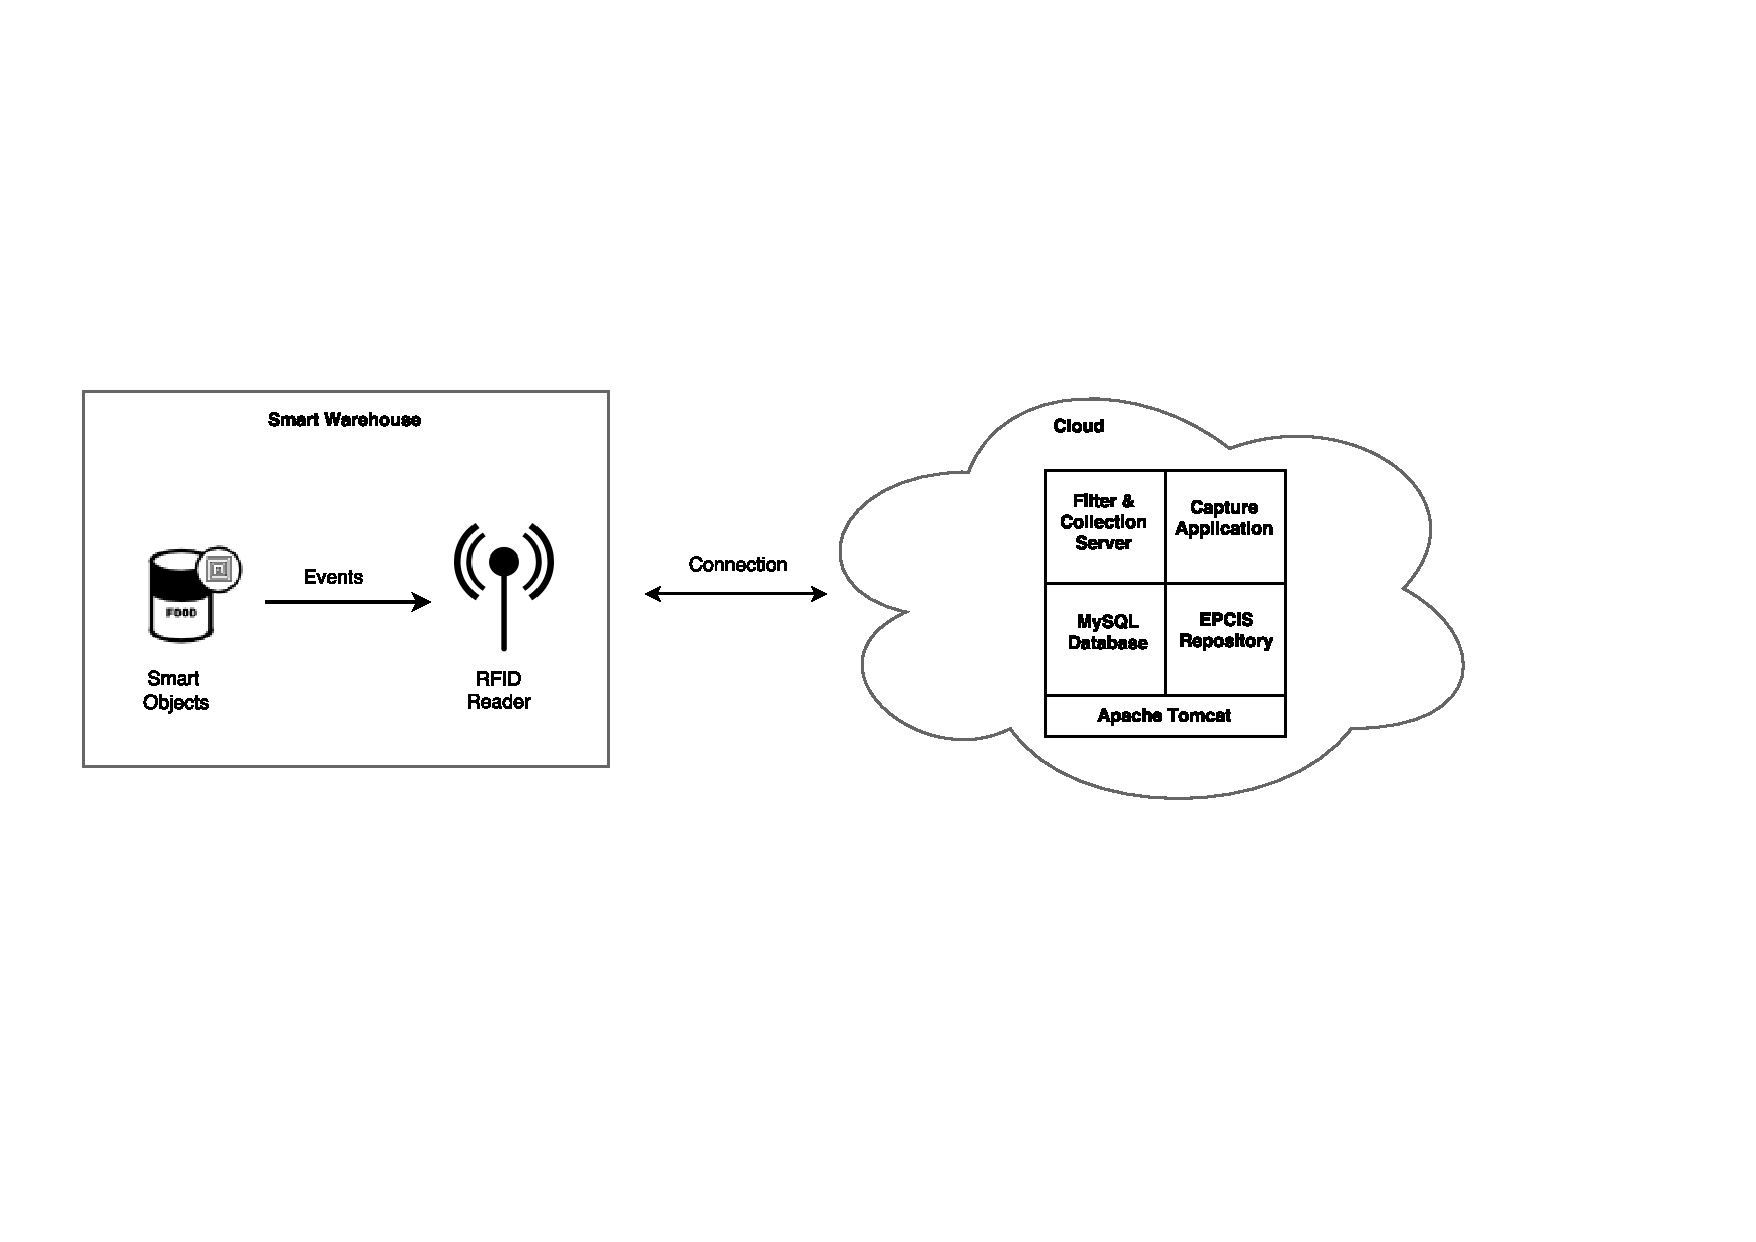
\includegraphics[width=\textwidth]{./images/implementation_cloud_architecture}
  \caption{Cloud-approach: smart warehouse technological architecture.}
  \label{fig:implementation_cloud_architecture}
\end{figure}

Figure~\ref{fig:implementation_cloud_architecture} presents the technological architecture for the cloud
approach. The \gls{RFID} middleware is provisioned in the cloud in a single virtual machine. In the
Fosstrak implementation the \gls{FCServer}, \gls{EPCIS} repository and the Capture application
requires an Apache servlet container to deploy and run the web applications. The \gls{EPCIS}
repository is connected to a MySQL database that stores the event data.\\

The smart warehouse is connected to the Fosstrak middleware through a Wi-Fi connection. The \gls{FCServer}
module periodically connect the readers to collect and process the events that were generated in the
warehouse.

% Fog approach
\subsection{Fog Deployment}
\label{sub:imp_smart_warehouse_fog}

% Fog approach
\begin{figure}[ht!]
  \centering
  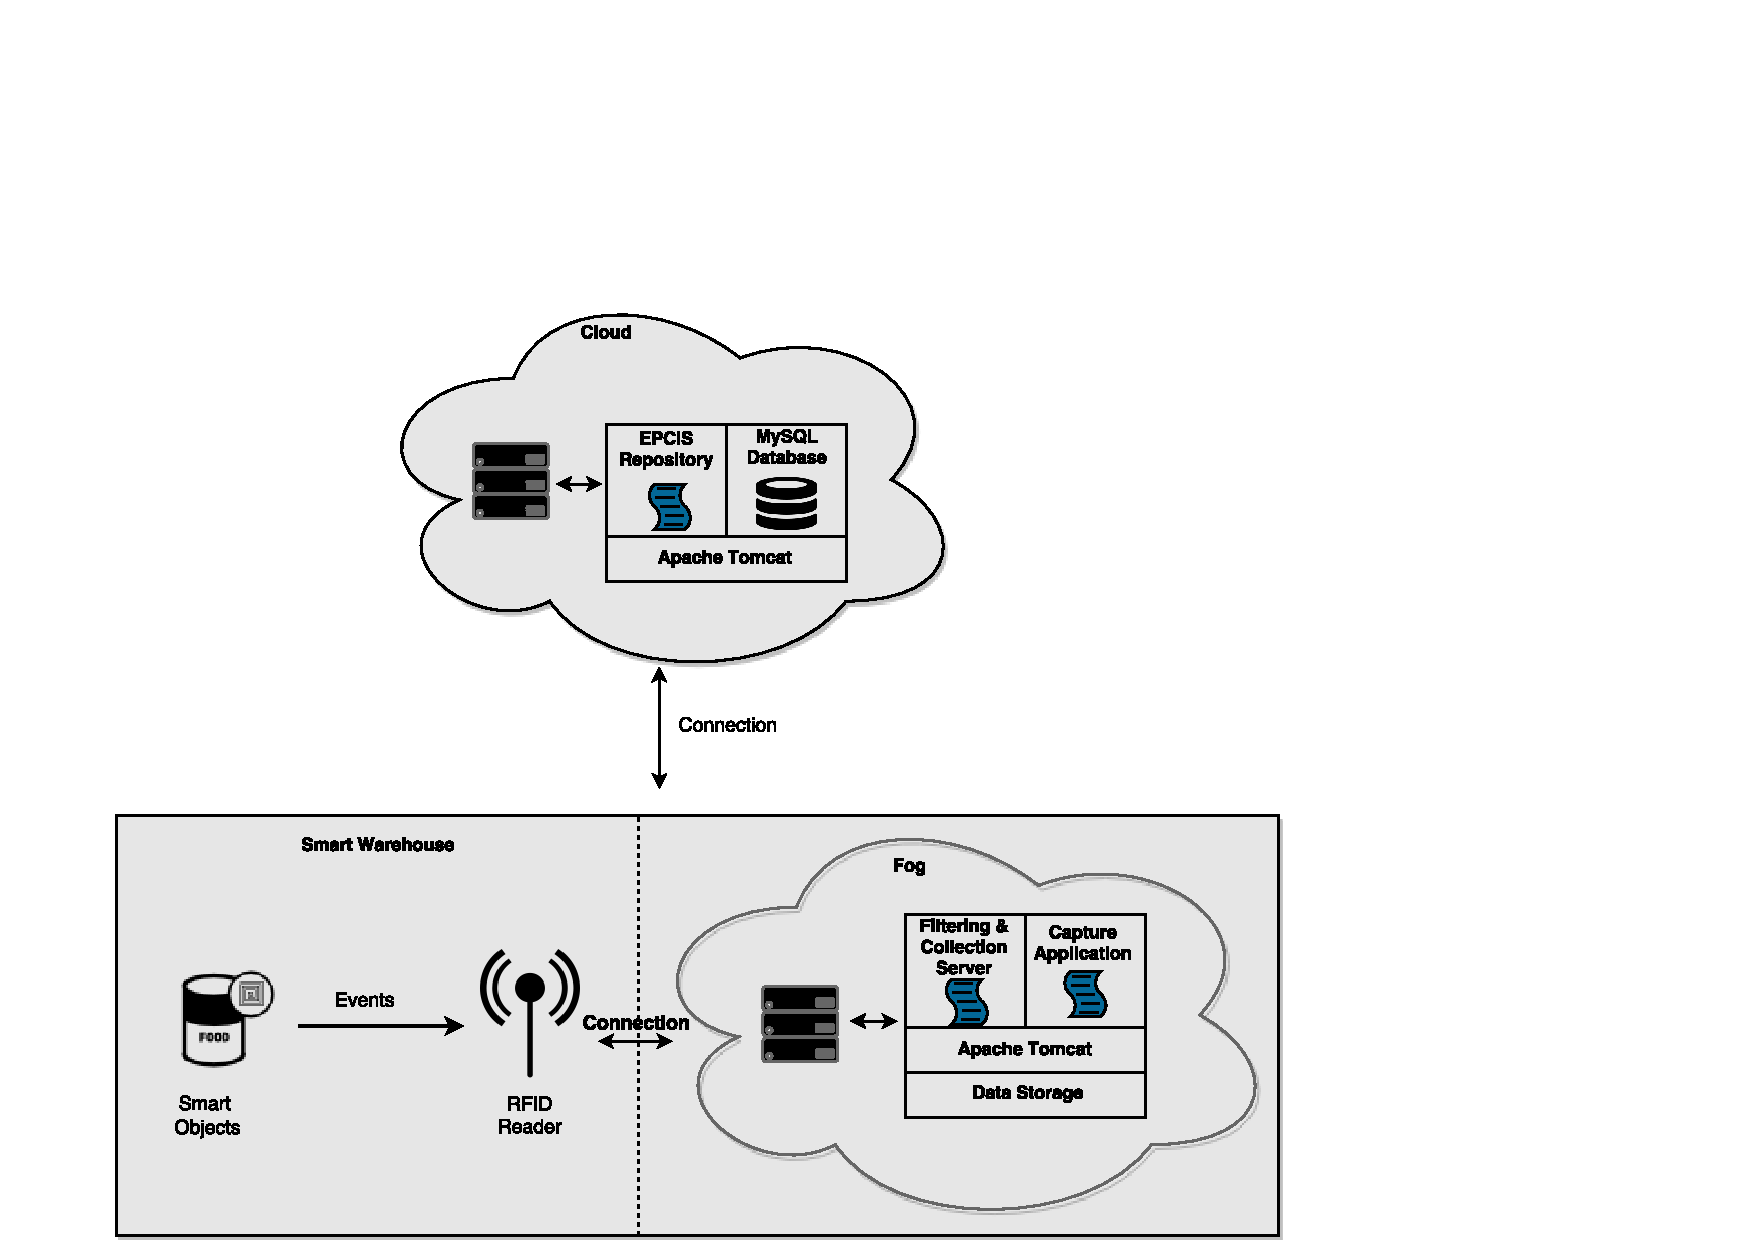
\includegraphics[width=\textwidth]{./images/implementation_fog_architecture}
  \caption{Fog-approach: smart warehouse technological architecture.}
  \label{fig:implementation_fog_architecture}
\end{figure}

Figure~\ref{fig:implementation_fog_architecture} presents the technological architecture for the fog
approach. The \gls{RFID} middleware is provisioned in the across the fog and the cloud in separated
virtual machines. In the cloud, the \gls{EPCIS} repository is deployed and running on top of an Apache
Tomcat servlet instance, and the repository is connected to a MySQL database. In the fog, the \gls{FCServer}
module and the Capture application are deployed and running on top of a single Tomcat servlet instance.
The Capture application sent the events collected by the \gls{FCServer} module to the \gls{EPCIS} repository
through the \textit{\gls{EPCIS} Capture Interface} - via \gls{HTTP} requests.\\

The connection between the smart warehouse and the fog is performed through a Wi-Fi connection, as
well the connection between the fog and the cloud.

\section{Provisioning}
\label{sec:provisioning}
The implementation of provisioning mechanism relies on the Chef tool. The recipes that describe our
infrastructure are based on cookbooks that are available on the Chef Supermarket. These recipes
describe how our software stack - are provisioned in the cloud instances. In the developed prototype,
we used Docker containers to provisioning the smart warehouse software in the cloud providers.
To provisioning the resources in the cloud instances instances we will use \textit{knife}, a command-line
tool developed by Chef that provides an interface between a local Chef repository and the Chef server.
The provisioning workflow is illustrated in Figure~\ref{fig:provisioning_tech_architecture}.\\ 

% Automatic provisioning diagram
\begin{figure}[!ht]
  \centering
  \makebox[\textwidth][c]{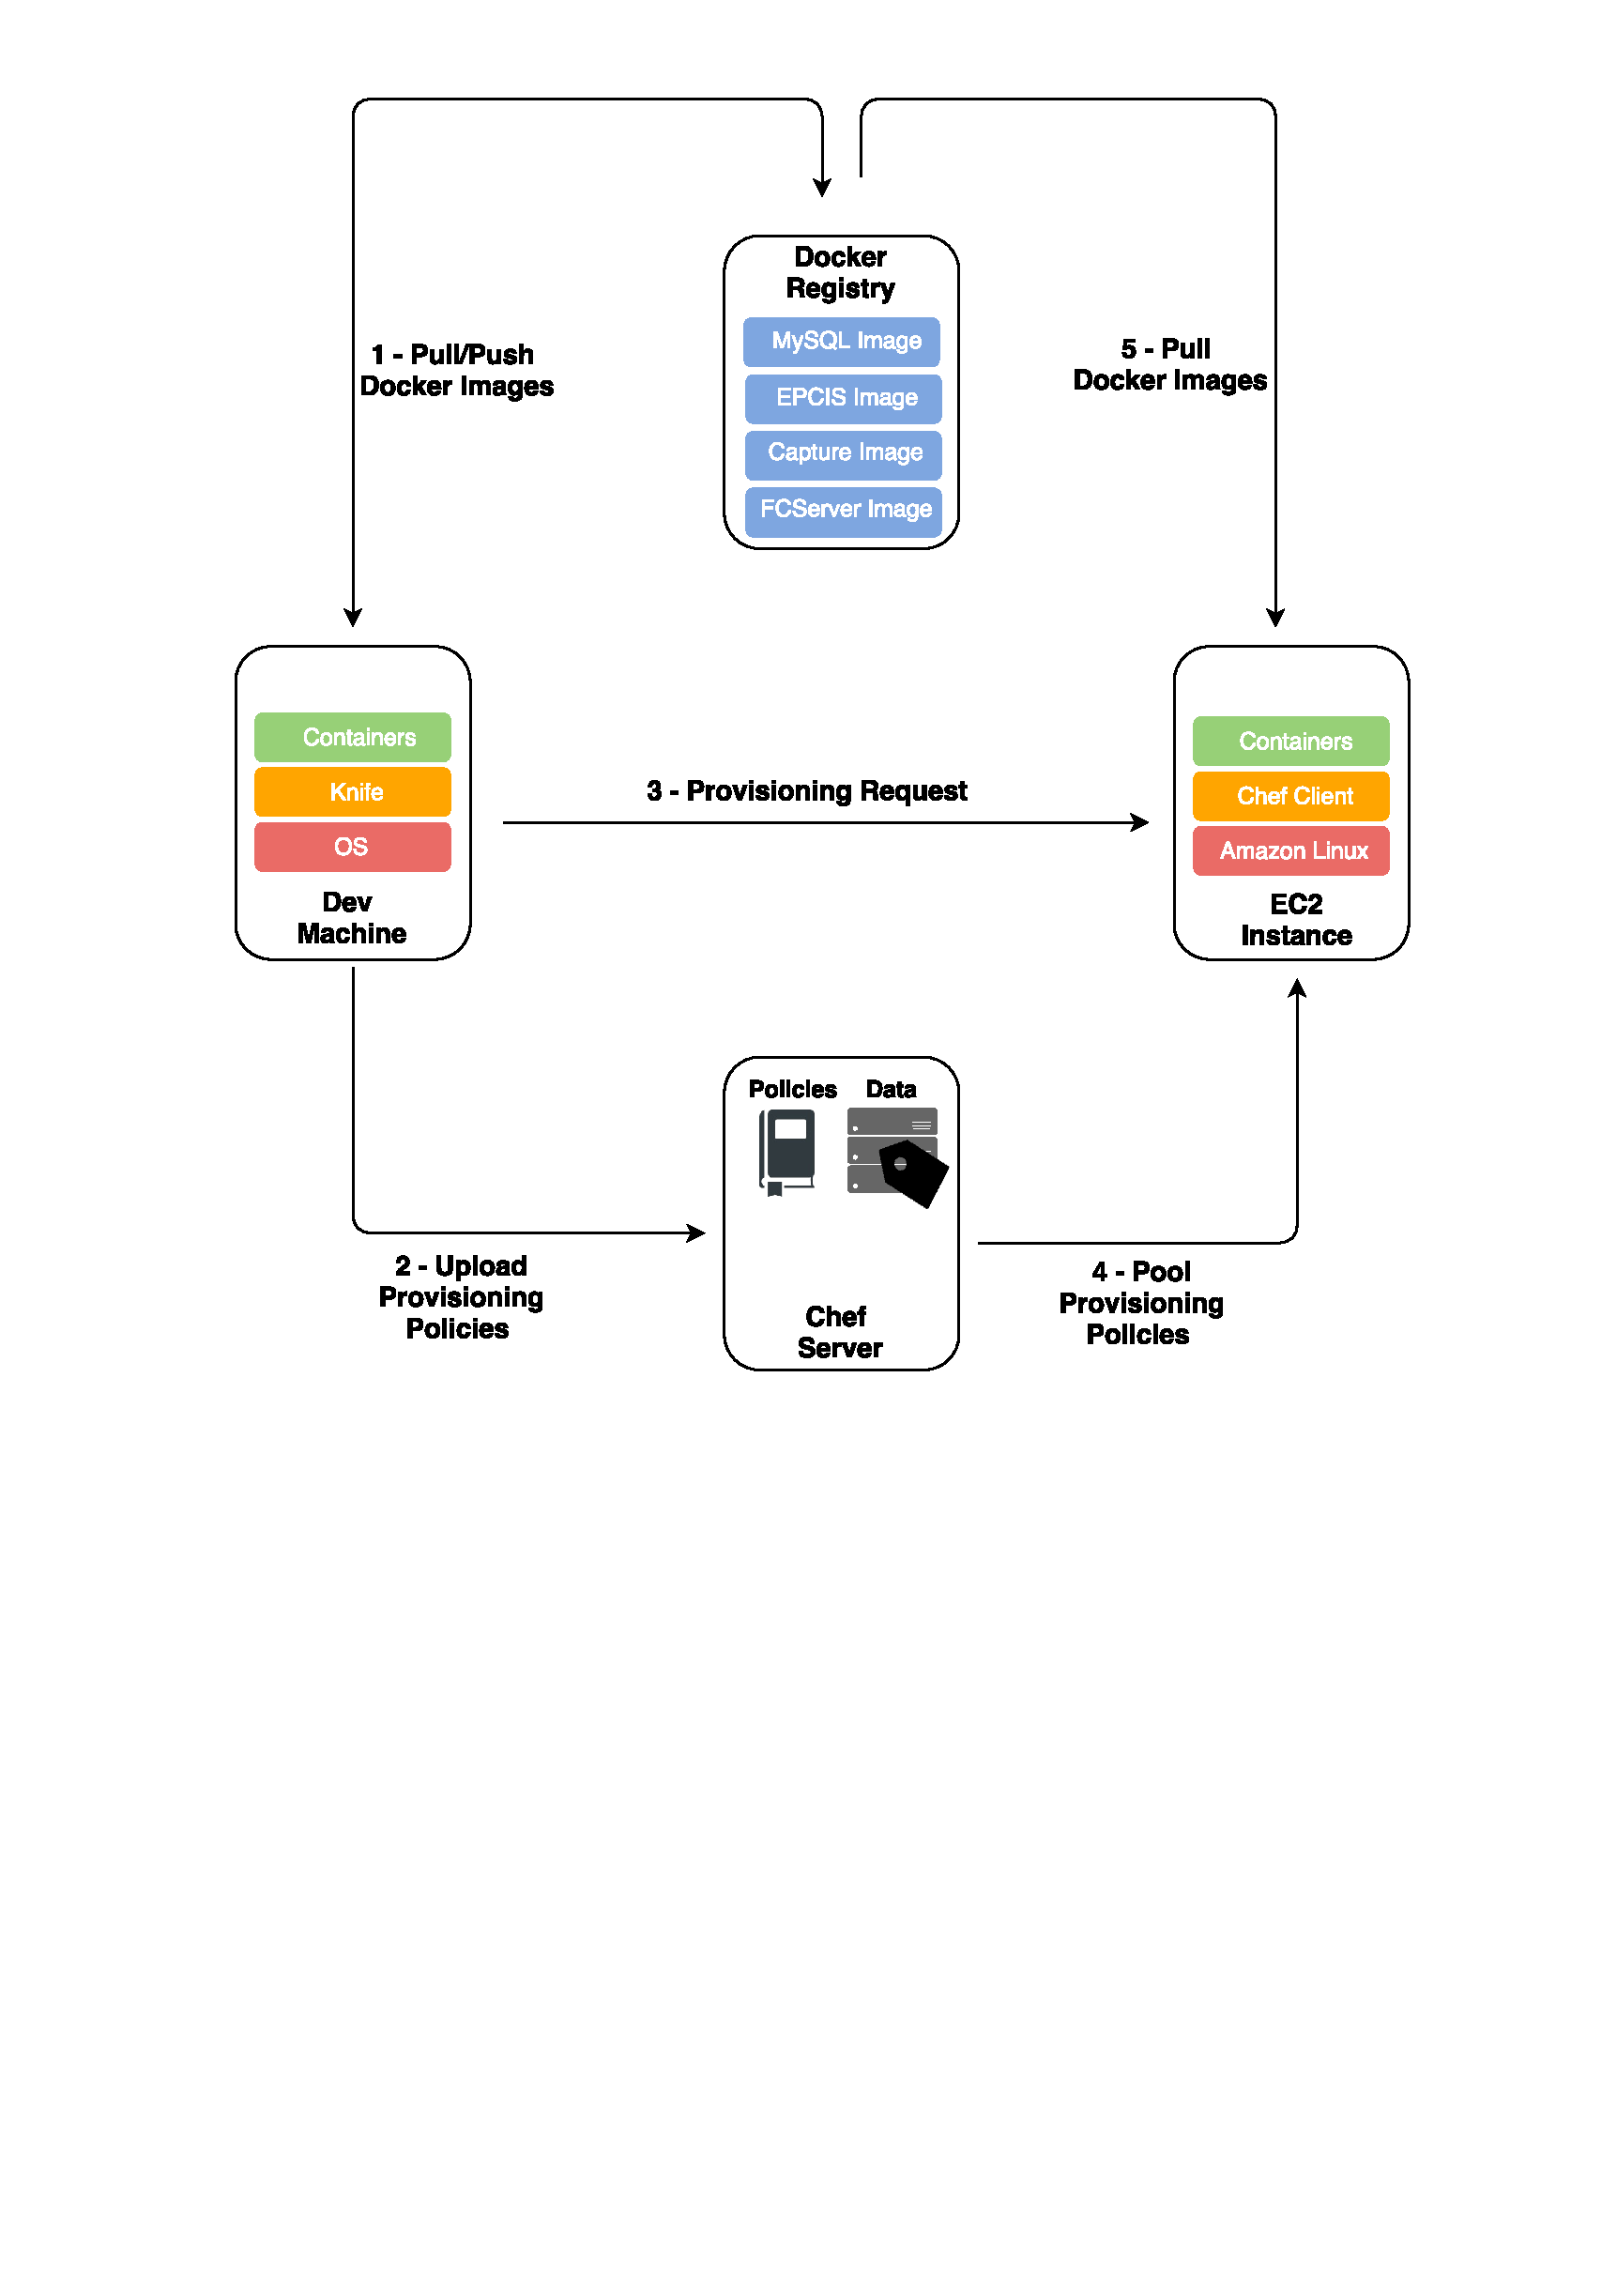
\includegraphics[width=.8\textwidth]{./images/c4t-tech-architecture}}%
  \caption{Automatic provisioning workflow.}
  \label{fig:provisioning_tech_architecture}
\end{figure}

In a development environment the Docker images are built and then uploaded to the Docker Registry
repository (1). The provisioning of the cloud resources is described in the cookbooks that are uploaded
to the Chef server (2). The provisioning request (3) is performed using \textit{knife}, that allows to
describe the image type, the instance type and the policies that need to be applied on each provisioned node.
Then the Chef client runs the configuration recipes that are pulled from the Chef server (4). In our
solution these configuration recipes describe that our nodes must have a set of Docker containers
running on it. The Chef client pulls the Docker images from the remote repository, build the containers
based on those images and finally applies the configuration that is associated to each container.

% Chef
\subsection{Chef}
\label{sub:impl_chef}
Chef is a configuration management tool that allows to describe the infrastructure as code.
In that way it is possible to automate how the infrastructure is built, deployed and managed.
Chef architecture is composed of the Chef Server - that stores the recipes and other configuration
data - and the Chef Client - that is installed in each server, \gls{VM} or container, i.e, the nodes that
are managed with Chef. The Chef client periodically pulls Chef server latest policy and state of the
network, and if anything on the node is out of date, the client update its state in order to be
consistent with the latest policy.\\

The tool was built from the ground with the cloud infrastructure in mind. With Chef, is possible to
dynamically provision and deprovision the application infrastructure on demand to keep up with
peaks in usage and track. For instance, \textit{knife} has a plugin for provisioning cloud resources
across several cloud providers - \gls{AWS}\footnote{https://aws.amazon.com/}, Google Compute
Engine\footnote{https://cloud.google.com/compute/} and Openstack\footnote{https://www.openstack.org/}.\\

We decide to chose Chef instead of its strongest competitors - i.e. Puppet and Ansible - for several
reasons, where the main one is \textit{knife}. \textit{knife} is very powerful and allow us to
interact with our entire infrastructure. For instance, it is possible to bootstrap a new server,
apply a role to a set of nodes in our environment. Furthermore, with \textit{knife ssh} it is
possible to execute a command on a certain any number of nodes in our environment.

% Docker containers
\subsection{Docker Platform}
\label{sub:impl_docker}
Docker containers are used to provisioning the software stack of the Fosstrak platform. A complete
installation of Fosstrak requires a compatible Java \gls{SDK}, a full MySQL database and a Apache Tomcat
server. In order to improve the application scalability we are provisioning a single container for each
component of the Fosstrak platform, the \gls{EPCIS} repository, the Capture application, the \gls{FCServer},
and also for the MySQL database. In our implementation, the container images of the Fosstrak stack
are published in the Docker Hub repository to later be used to create the containers.\\

By default each container runs a process that is isolated from the other processes that are executed
in the same environment. In order to connect the different modules of the Fosstrak, our containers are
linked through the \textit{linking system} provided by Docker. This mechanism creates a secure tunnel
between the containers, allowing the recipient container to access select data about the source container.
For instance, if we have a web server container linked to a database container, the web server container
is able to access information about the database container.\\

The reasons to chose Docker containers instead of traditional \glspl{VM} is that containers are a
virtualization platform which its images requires less disk space and I/O when compared with traditional
\gls{VM} images \cite{merkel2014docker}. Furthermore, Docker containers are portable, which means that
they can be moved across different infrastructures depending on how the application scales.
